% Created: 2019-12-10
% Plot participant data
% http://github.com/zhaobn/magic_stones

\documentclass{article}
\title{[Magic Stones] Participant data visualization}
\author{Bonan Zhao (b.zhao@ed.ac.uk)}

% Text formats: margin, font, spacing
\usepackage[margin=0.8in]{geometry}
\usepackage{charter}
\renewcommand{\baselinestretch}{1.3}

% Graphics
\usepackage{graphicx}
\usepackage{subcaption}
\graphicspath{{../figs/}}


\begin{document}
\maketitle


\begin{figure}[b]
	\centering
  \begin{subfigure}[t]{0.31\textwidth}
  	\centering
  	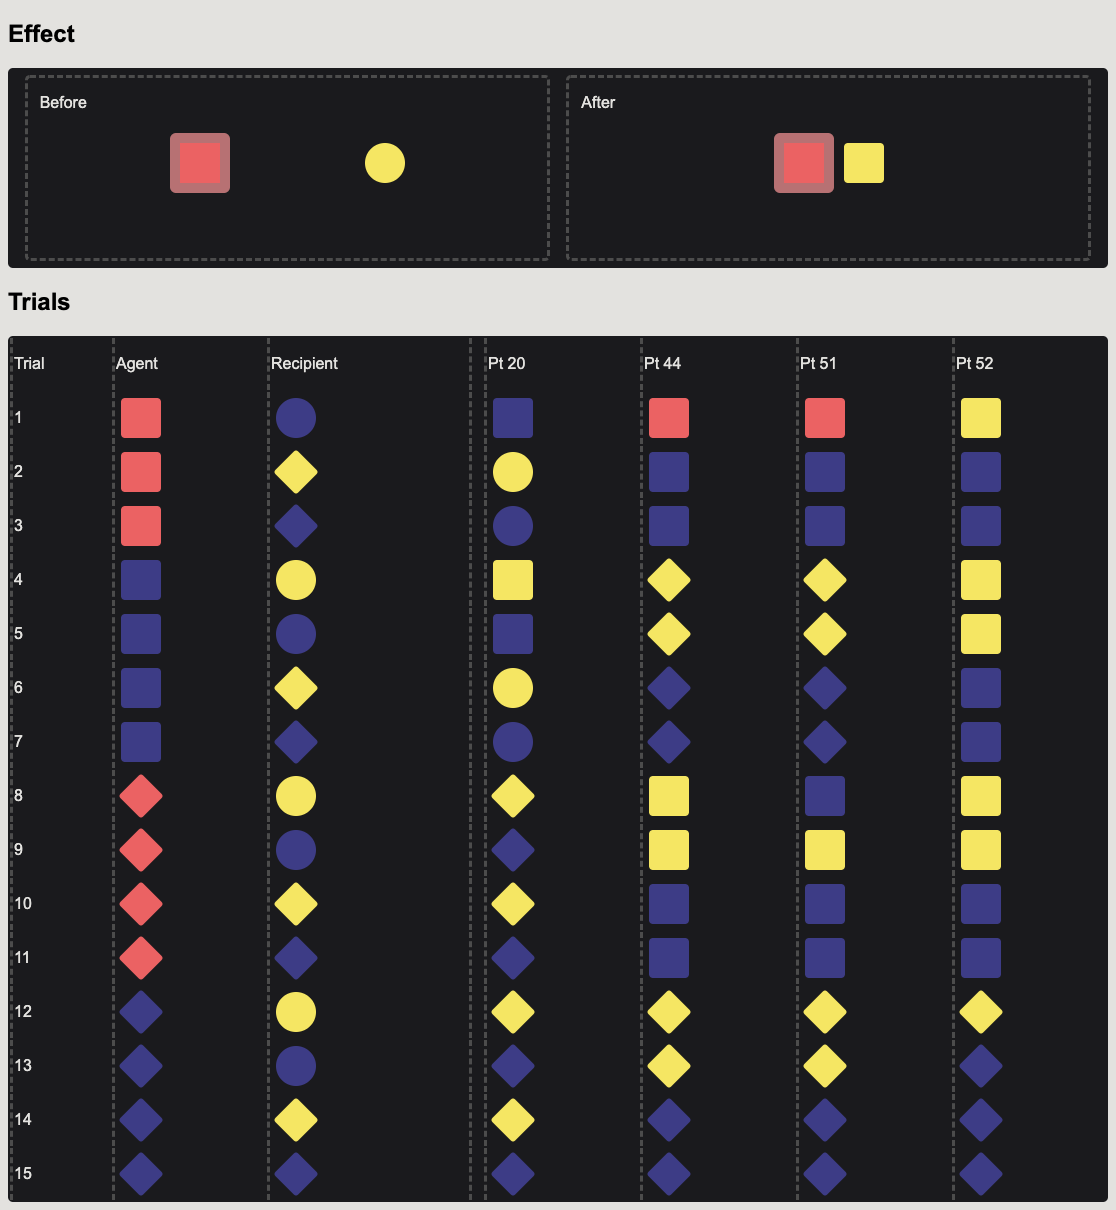
\includegraphics[width=\linewidth]{group01} 
  	\caption{To the same shape} \label{fig:group01}
  \end{subfigure}
  \hfill
  \begin{subfigure}[t]{0.31\textwidth}
  	\centering
  	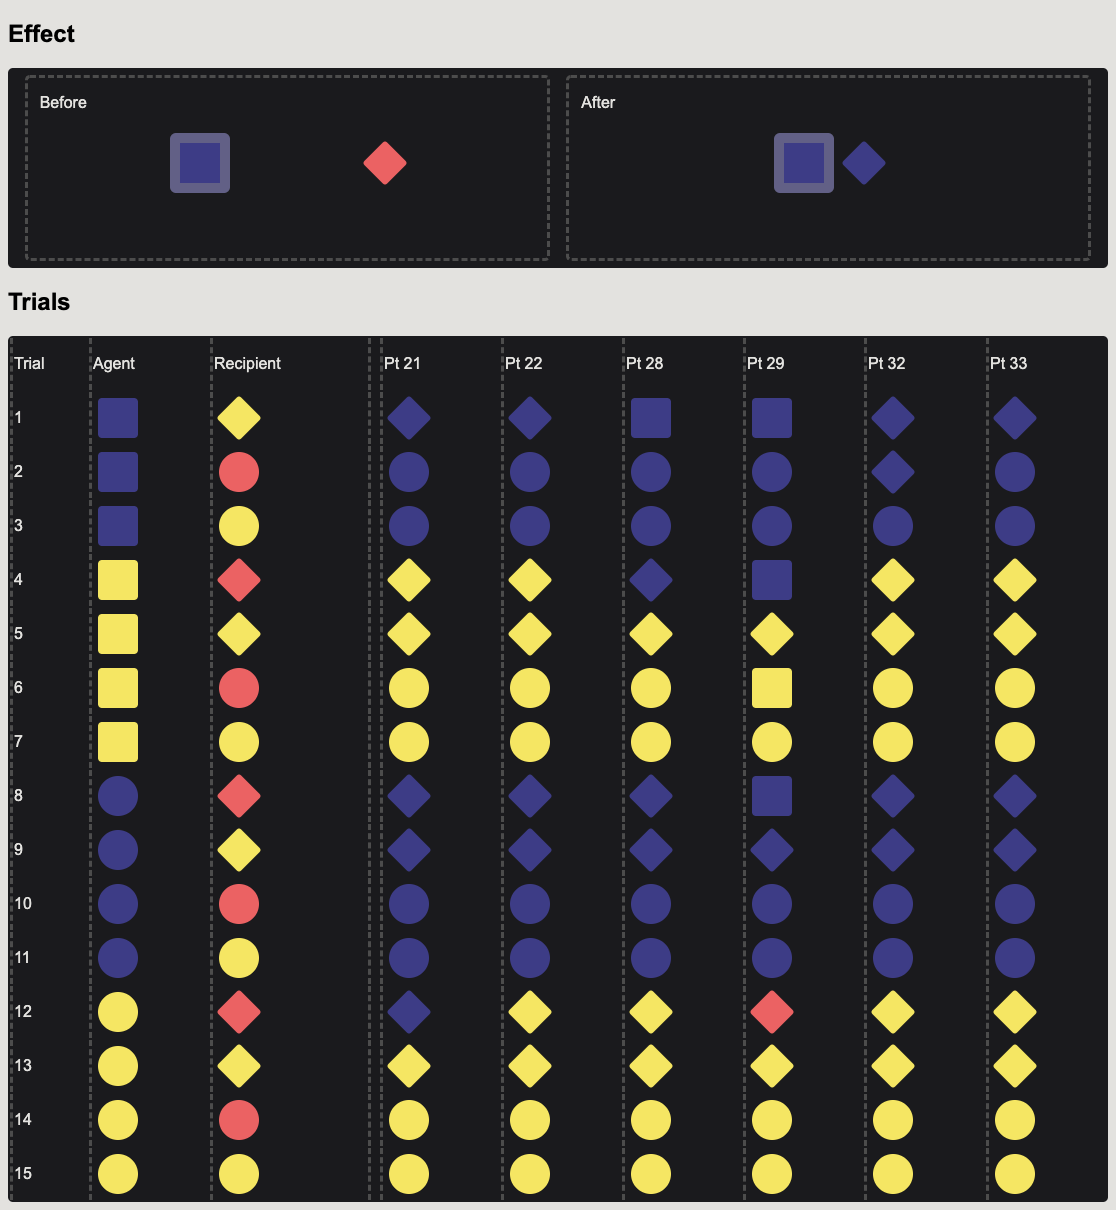
\includegraphics[width=\linewidth]{group03} 
  	\caption{To the same color} \label{fig:group03}
  \end{subfigure}
  \hfill
  \begin{subfigure}[t]{0.31\textwidth}
  	\centering
  	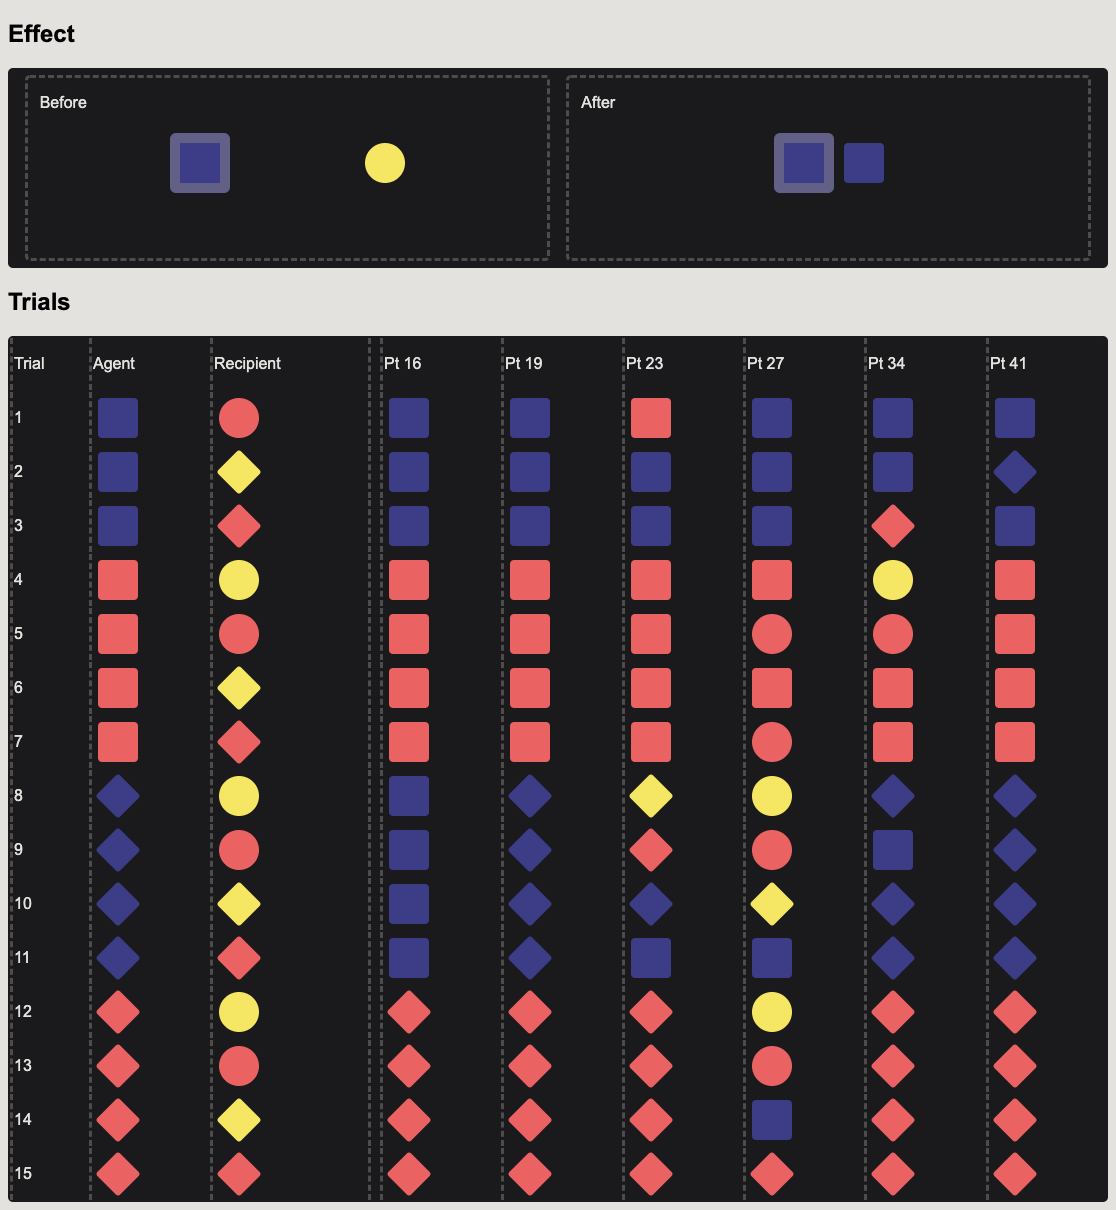
\includegraphics[width=\linewidth]{group06} 
  	\caption{To the same object} \label{fig:group06}
  \end{subfigure}

  \vspace{1cm}
  \begin{subfigure}[t]{0.31\textwidth}
  	\centering
  	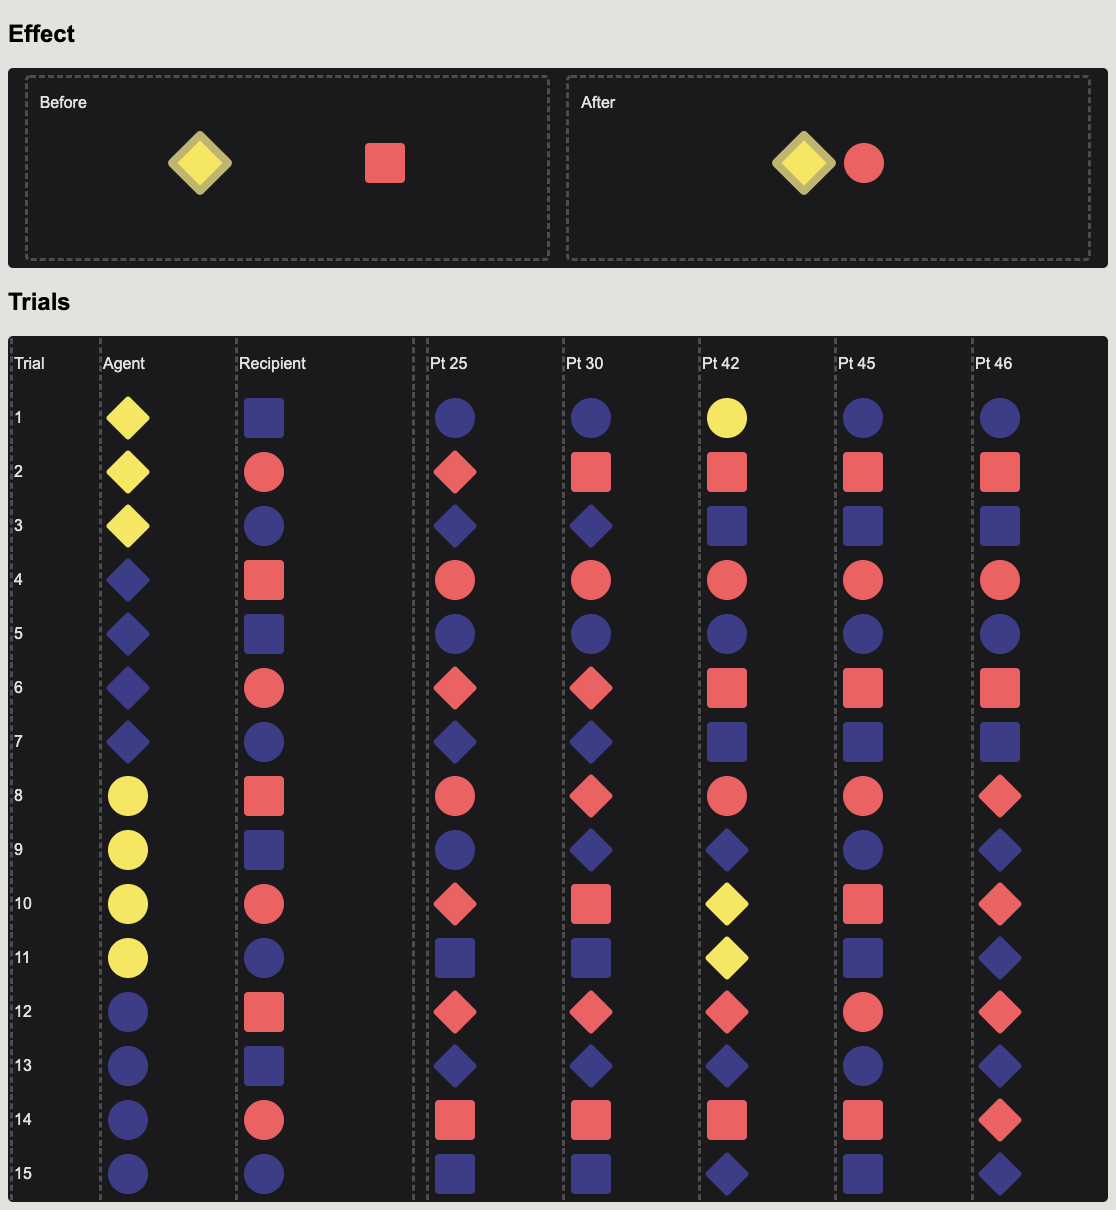
\includegraphics[width=\linewidth]{group02} 
  	\caption{To a different shape} \label{fig:group02}
  \end{subfigure}
  \hfill
  \begin{subfigure}[t]{0.31\textwidth}
  	\centering
  	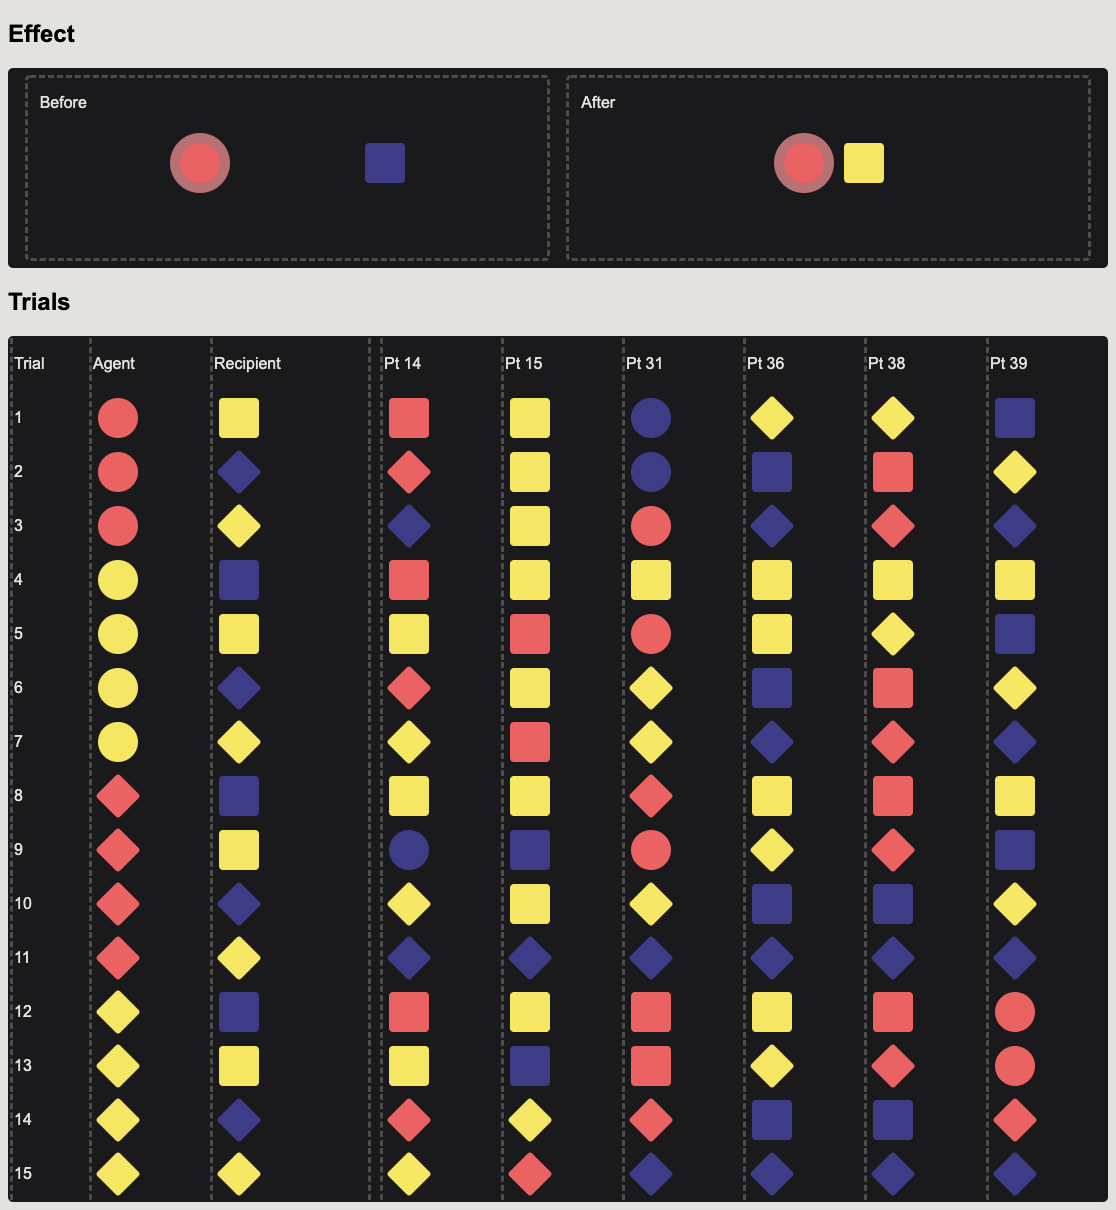
\includegraphics[width=\linewidth]{group04} 
  	\caption{To a different color} \label{fig:group04}
  \end{subfigure}
  \hfill
  \begin{subfigure}[t]{0.31\textwidth}
  	\centering
  	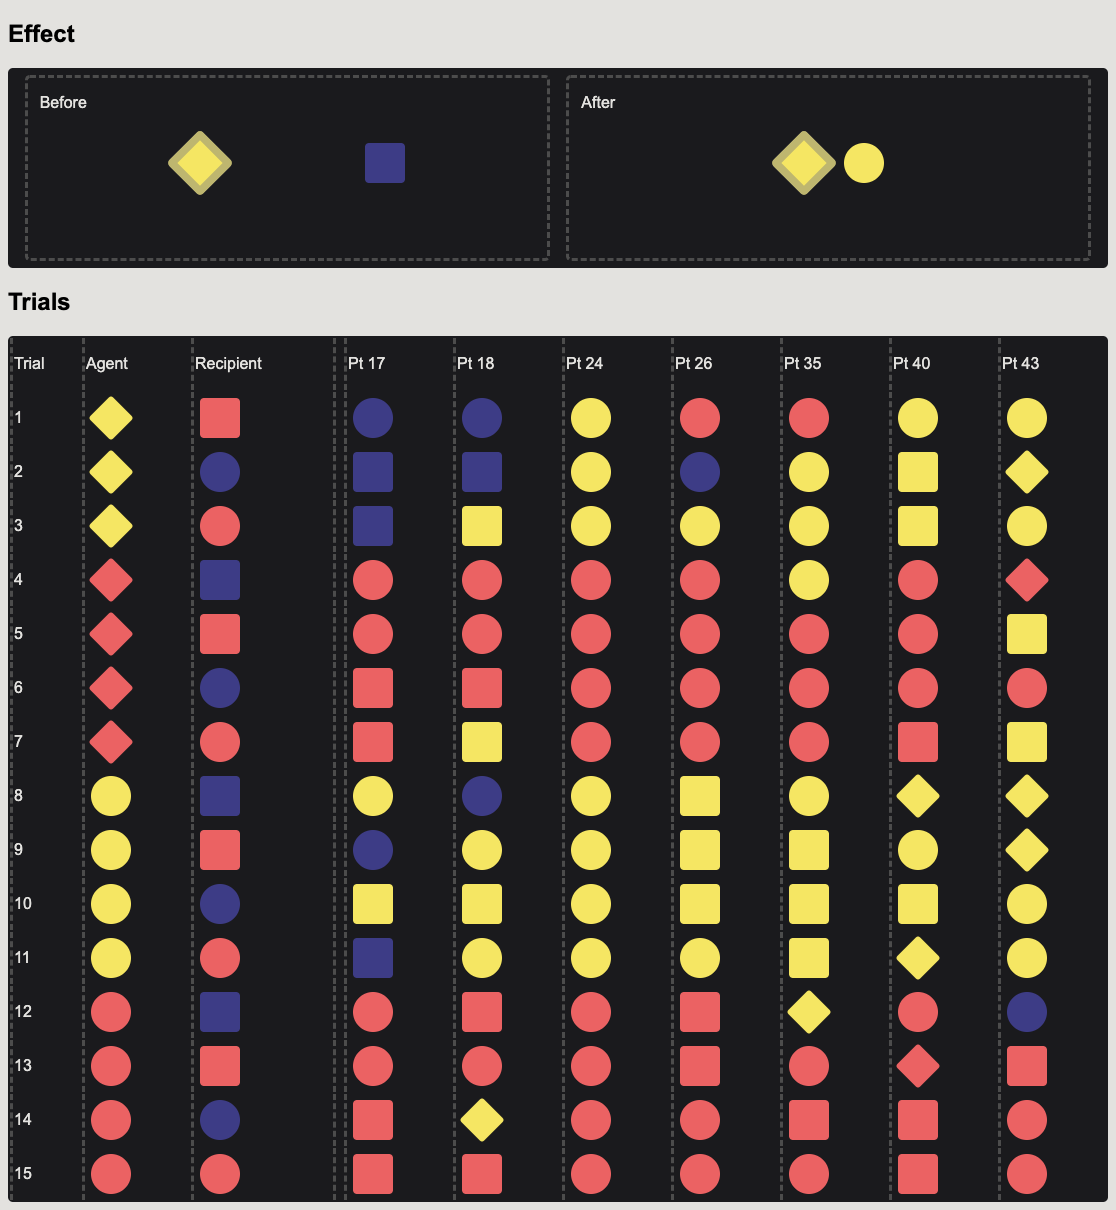
\includegraphics[width=\linewidth]{group05} 
  	\caption{To a different object} \label{fig:group05}
  \end{subfigure}
  \caption{Some general caption of all the figures. In (\subref{fig:group01}) you can see a  green square....}
\end{figure}




\end{document}